\section{Performance of the Spherical Harmonics Analysis in Separating 0\nbb-decay from \B~Background.}
\label{sec:performance}

In this section we discuss factors that affect performance of the spherical harmonics analysis in separating
0\nbb~signal from \B~background events. We found that most separation comes from the first two multiple moments,
$l=0$ and $l=1$. However, according to Eq.~\ref{eq6}, higher multiple moments are needed for a better normalization of the 
power spectrum $S_l$. In the following we choose to calculate power spectrum $s_l$ up to multiple moment of l=3 and
use only normalized variable $S_0$ and $S_1$, where the normalization is given by

\begin{eqnarray}
\label{eq7}
S_{0,1} = \frac{s_{0,1}}{\sum_{l=0}^{3} s_l}
\end{eqnarray}

As discussed below, a linear combination of $S_0$ and $S_1$ can be used to construct a single variable, $S_{01}$, that provides 
separation between signal and background in 1-D space. We show distributions of this variable $S_{01}$ to demonstrate qualitatively 
the separation between 0\nbb~and \B~events depending on a few key assumptions about the detector characteristics.

Since the goal of this paper is to describe the technique of spherical harmonics analysis for separating
different event topologies relevant for 0\nbb-decay searches in a generic liquid scintillator detector, we intentionally refrain from any 
quantitative estimates on the improvements in sensitivity to 0\nbb~decay. The actual improvements in sensitivity due to spherical 
harmonics analysis would depend on various details of a given experimental setup. Therefore, we believe that detailed quantitative 
sensitivity studies are more appropriate in the context of a particular 0\nbb~decay experiment which is beyond the scope of this paper.

\subsection{Central events with perfect vertex reconstruction}

We start evaluating the performance of the spherical harmonics analysis by looking at events that originate at the center
of the detector and by assuming perfect reconstruction of the event vertex position. For such events, a time cut of 33.5~ns on PEs 
arrival time can be applied to obtain early PEs sample which contain high fraction of Cherenkov PE. The default QE and 100\% 
photo-coverage is used in the simulation.

Comparison of $S_0$ and $S_1$ distributions for 0\nbb-decay signal and \B~background events is shown in Fig.~\ref{fig:S_vs_energy}.
Both variables provide a noticeable separation between signal and background. We also note that in the energy range of interest, 
the $S_l$'s do not strongly depend on the energy deposited in the detector, which makes information contained in the normalized power 
spectrum complimentary to the energy measurements. Therefore, spherical harmonics analysis can be used as an additional handle for
background suppression at the end point of the 0\nbb-decay energy spectrum.

\begin{figure*}[h]
\centering
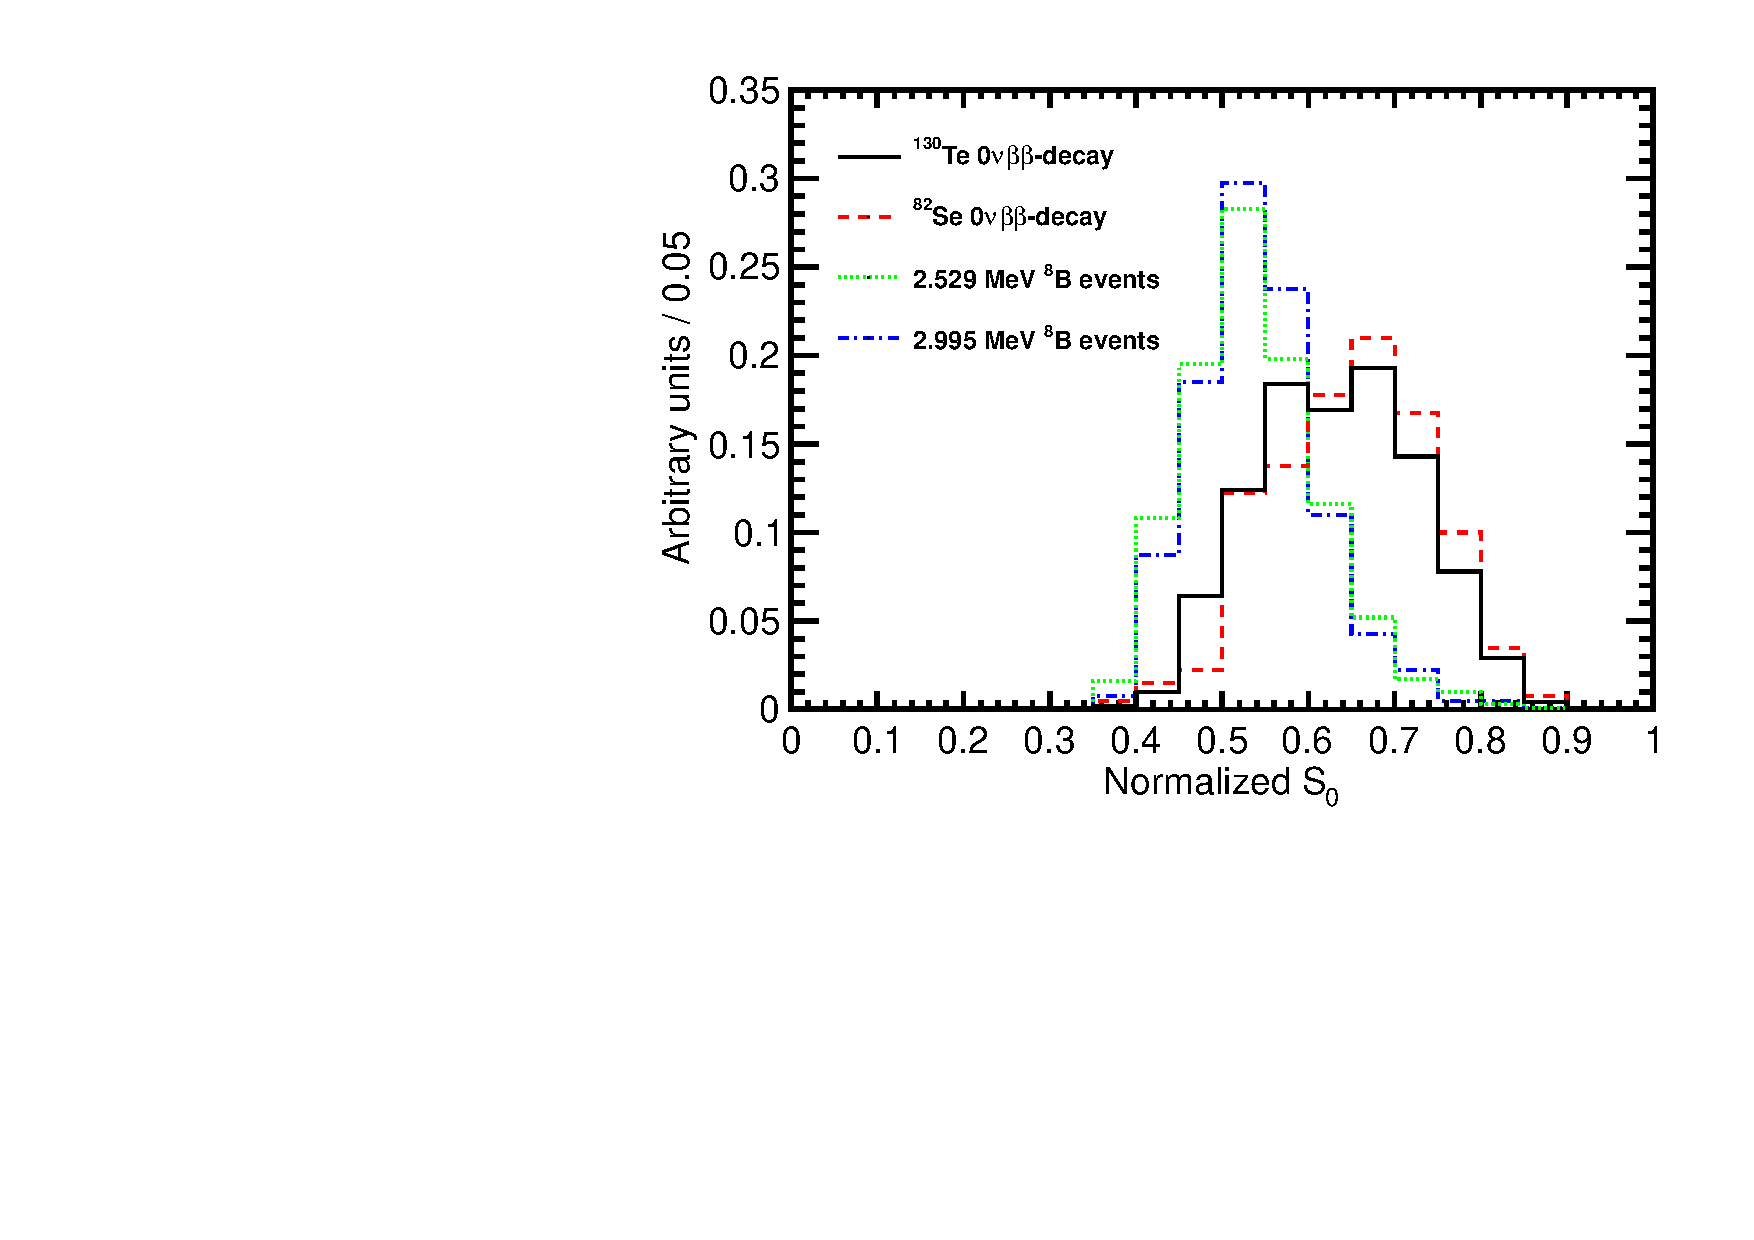
\includegraphics[width=0.49\textwidth]{hS0.pdf}
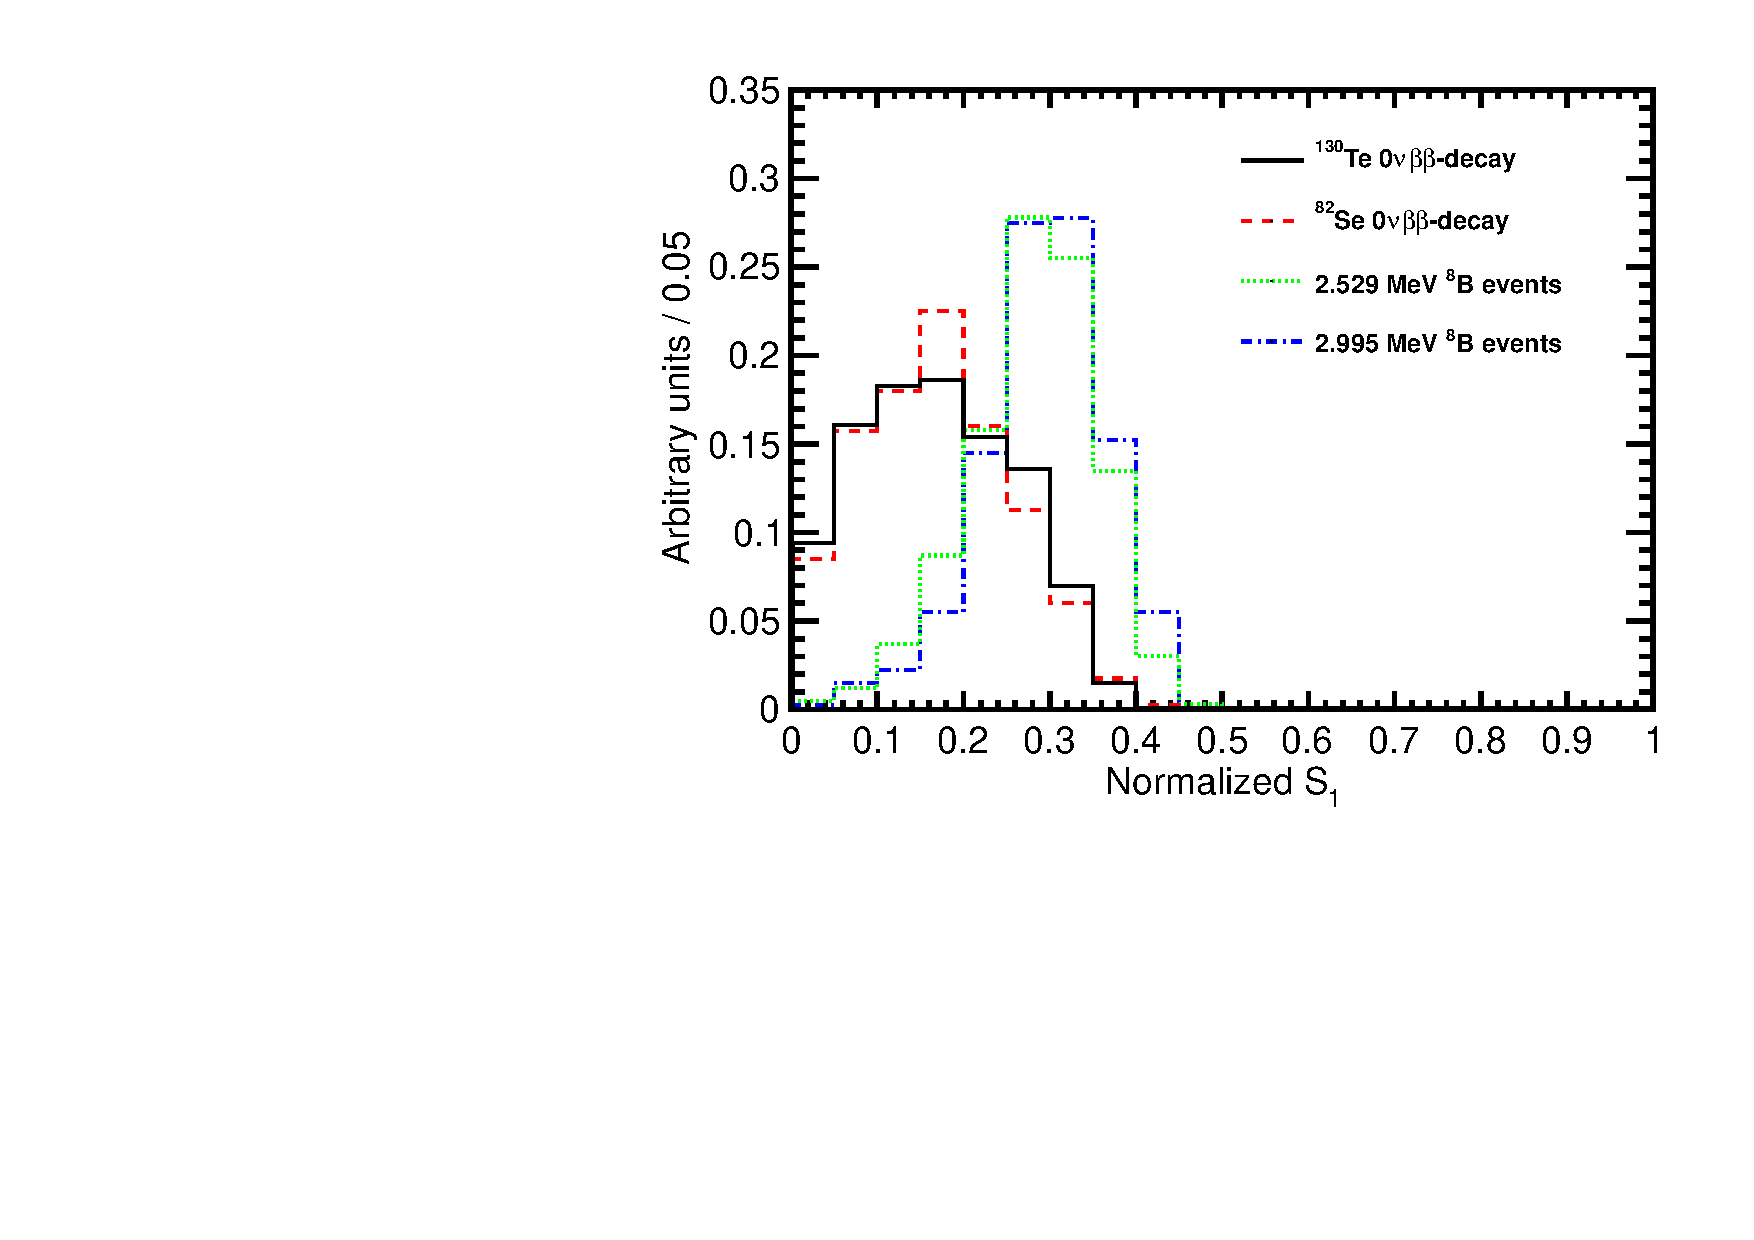
\includegraphics[width=0.49\textwidth]{hS1.pdf}
\caption{$S_0$ (\emph{left}) and $S_1$ (\emph{right}) distributions for 1000 simulated 0\nbb-decay signal and \B~background events.
  Two different isotopes are compared, $^{130}$Te and $^{82}$Se. Corresponding kinetic energies of \B~single electrons are
  2.53 MeV and 3.00 MeV. Central events assuming perfect reconstruction of vertex position. Time cut of 33.5~ns on the PE arrival time is
  applied. The default QE and 100\% photo-coverage is used in the simulation.}
\label{fig:S_vs_energy}
\end{figure*}

Left panel in Fig.~\ref{fig:SL_Te_33p5ns_center} compares scatter plots of the first two components of the power spectrum, 
$S_0$ and $S_1$, for signal and background. In order to optimize separation between $^{130}$Te and $^{8}$B
events, a linear combination of variables $S_0$ and $S_1$ is constructed as follows. 

First, a linear fit, $S_0$ = $A \cdot S_1 + B$, of all points on the scatter plot is performed as shown by the dashed 
line in the left panel in Fig.~\ref{fig:SL_Te_33p5ns_center}. Then a 1-D variable $S_{01}$ is defined as
$S_{01} = S_1 \cdot cos(\theta) + S_0 \cdot sin(\theta)$, where $tan(\theta)$=$A$. Right panel in Fig.~\ref{fig:SL_Te_33p5ns_center}
compares distributions of $S_{01}$ for 0\nbb-decay signal and \B~background. These 1-D histograms for $S_{01}$ represent
projection of the points on the scatter plot onto the fitted line. We use distribution of the variable $S_{01}$ as a figure of merit
for signal/background separation. Figure~\ref{fig:SL_Te_33p5ns_center} demonstrates that spherical harmonics analysis potentially 
brings extra separation power which\ is in addition to the energy measurements.


\begin{figure*}[h]
  \centering
  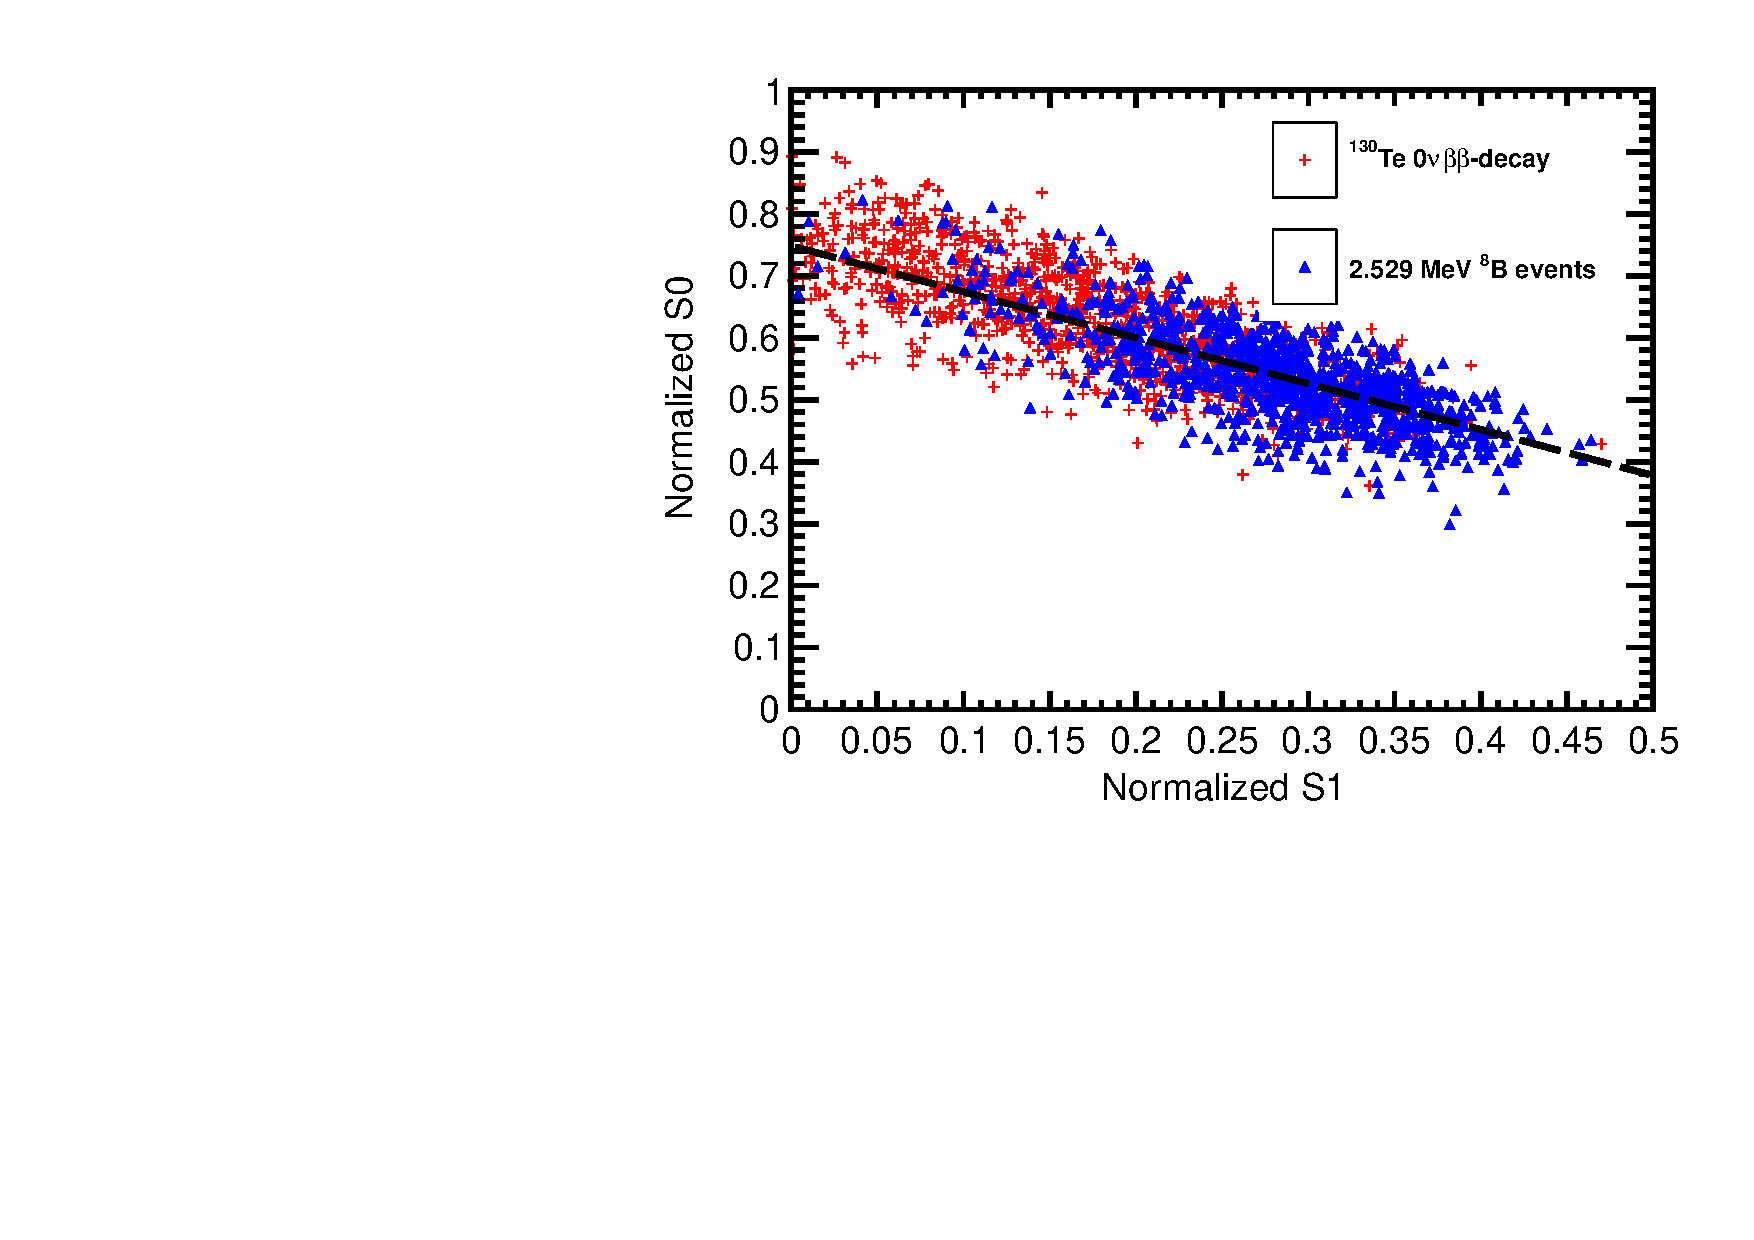
\includegraphics[width=0.49\textwidth]{hS0vsS1_Te130_1el_allLight_VtxSmear0cm_VtxShiftX0cm_33p5ns_center.pdf}
%  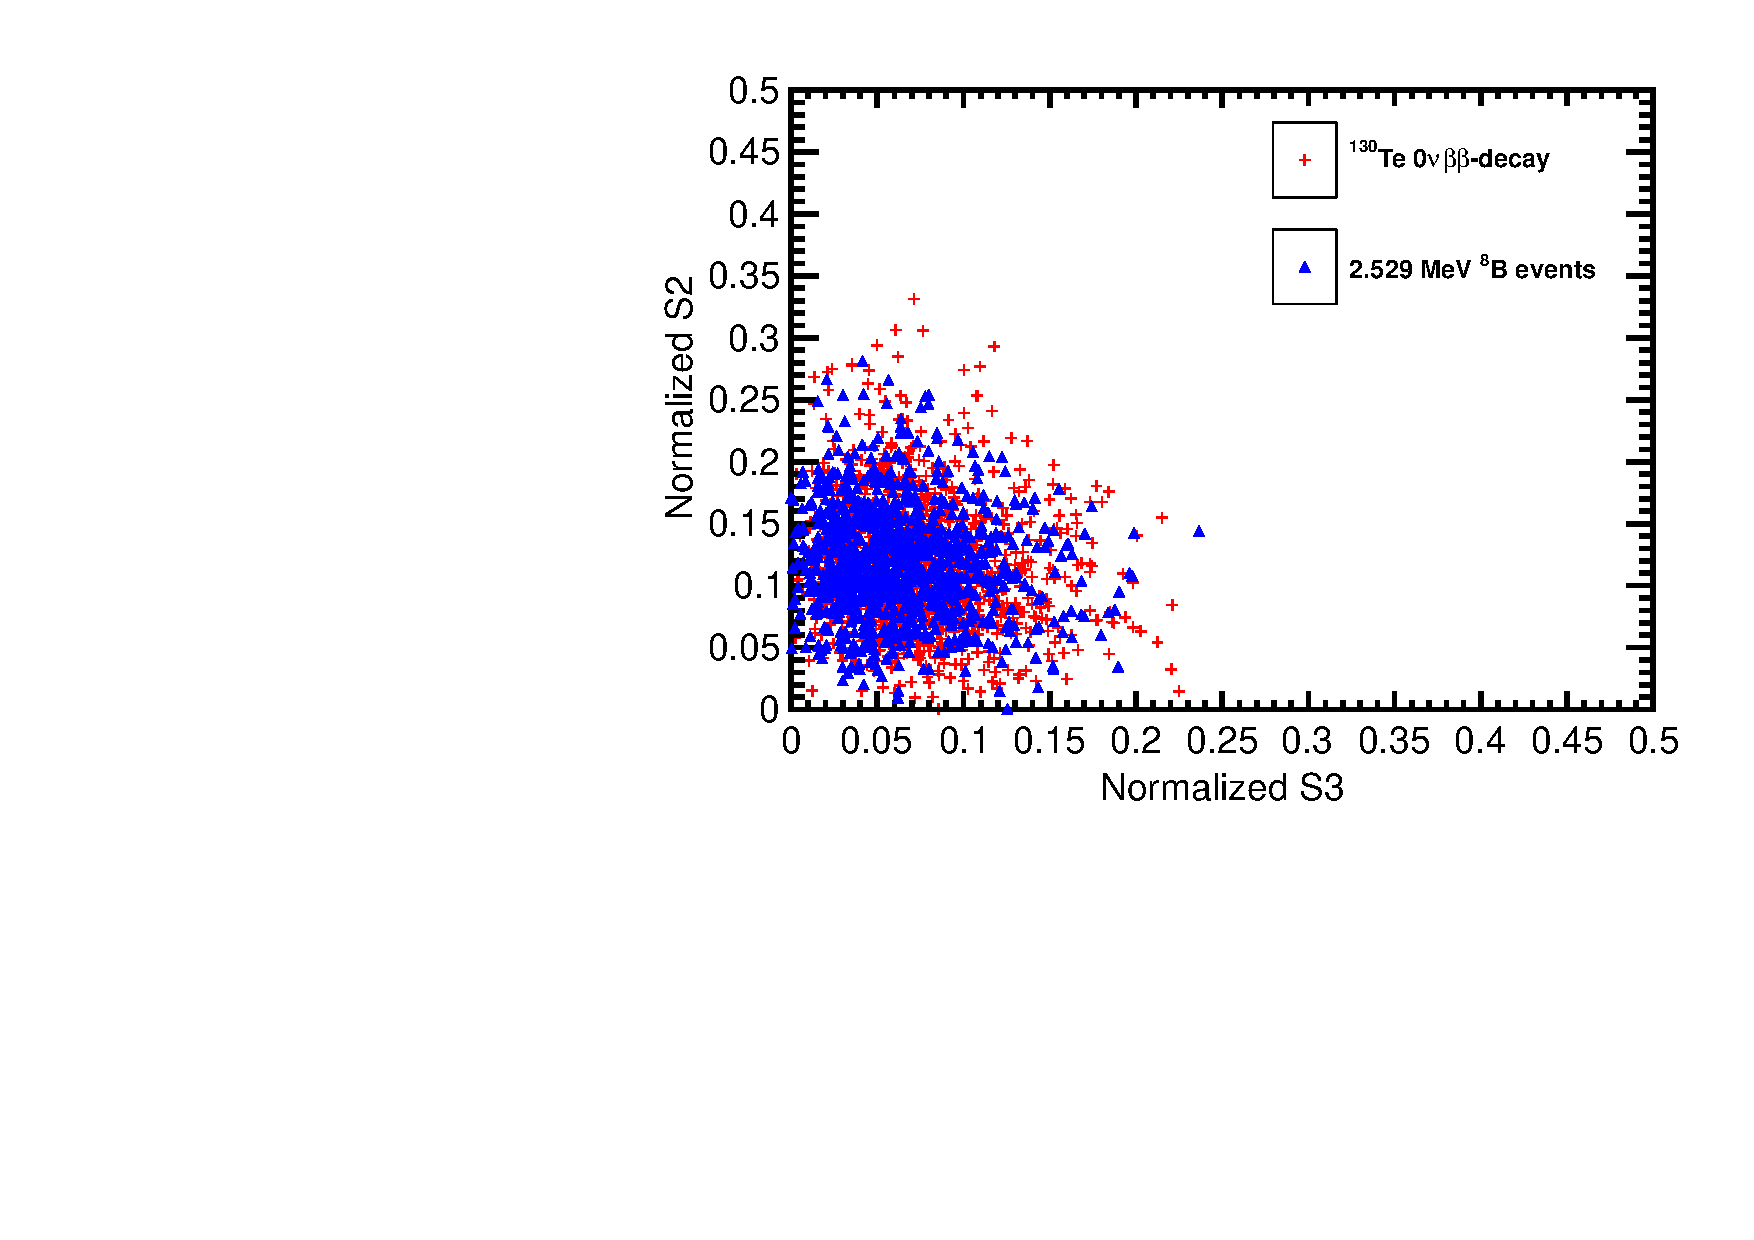
\includegraphics[width=0.49\textwidth]{hS2vsS3_Te130_1el_allLight_VtxSmear0cm_VtxShiftX0cm_33p5ns_center.pdf}
  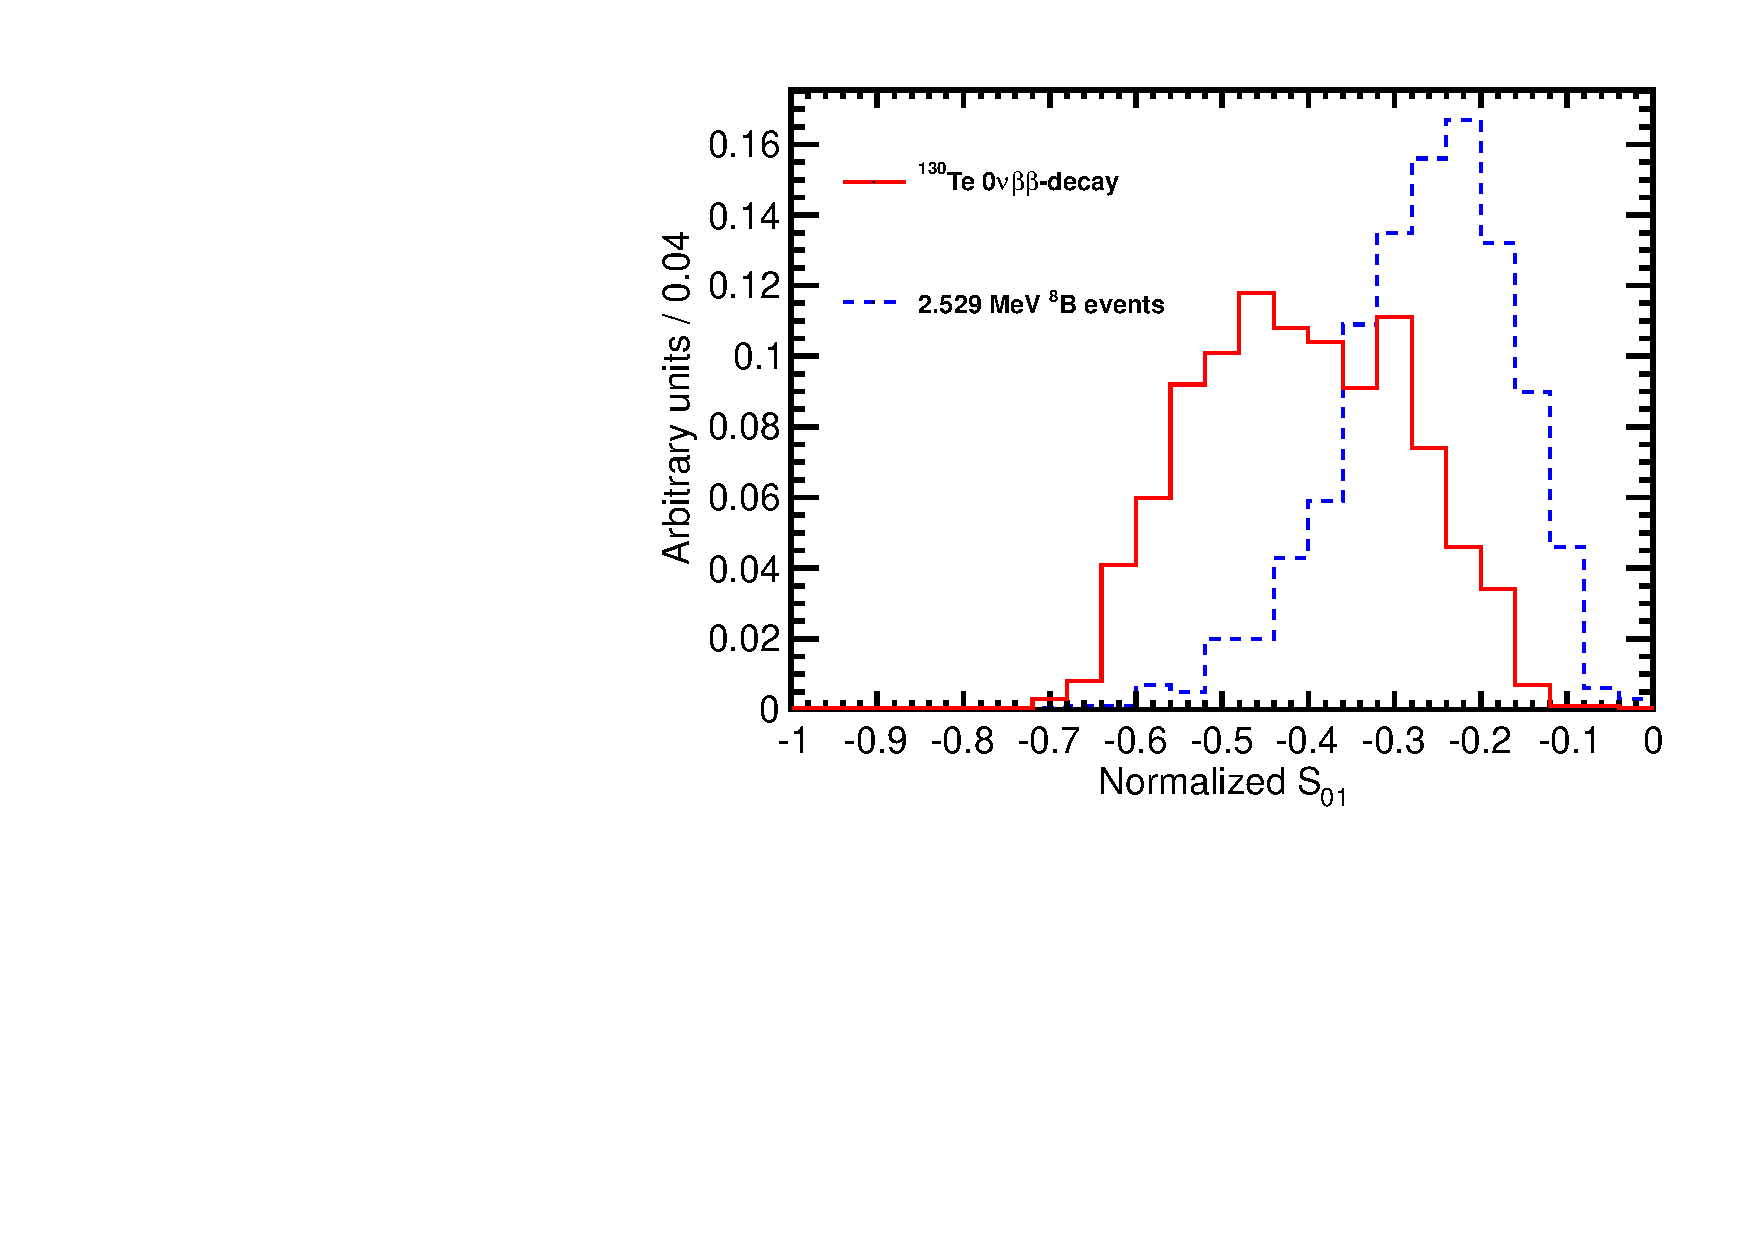
\includegraphics[width=0.49\textwidth]{hS01_allLight_VtxSmear0cm_VtxShiftX0cm_33p5ns_center.pdf}
  \caption{\emph{Left:} Scatter plot of $S_0$ versus $S_1$ for a simulation of 1000 signal (\emph{red crosses}) and background 
    (\emph{blue triangles}) events.
    Central events assuming perfect reconstruction of vertex position. Time cut of 33.5~ns on the PE arrival time is
    applied. The default QE and 100\% photo-coverage is used in the simulation.
    Black dashed line corresponds to a linear fit to define 1-D variable $S_{01}$ (see text for details).
    \emph{Right:} Comparison of the $S_{01}$ distribution between signal (\emph{red solid line}) and background (\emph{blue dashed line}).}
\label{fig:SL_Te_33p5ns_center}
\end{figure*}



\subsection{Experimental challenges}

So far only events at the center of the detector have been considered. Precise vertex reconstruction has been also assumed. 
Here we discuss performance of the spherical harmonics analysis for events that originate throughout the whole fiducial volume
of the detector and that also have limited vertex reconstruction precision.

Selection of early PE sample using absolute time cut of 33.5~ns that has been applied to central events relies on the fact that, 
within the uncertainty on electron track length, all photons travel the same distance before reaching the surface of the detector. 
PEs with early measured time correspond mostly to Cherenkov photons because of the delay in the scintillation process and longer 
wavelength of the Cherenkov light. 

When the vertex is not at the center, a uniform absolute time cut on the photon arrival time is no longer effective in selecting 
Cherenkov photons. In the case of an off-center vertex, there could be a situation when even significantly delayed scintillation photons 
reach the side of the detector that is closer to the vertex much earlier than Cherenkov photons traveling to the opposite side of the 
detector. Therefore, the time cut has to take into account the total distance traveled by each individual photon.

We found that a differential time cut defined as $\Delta t=t^{phot}_{measured} - t^{phot}_{predicted}<$1~ns selects photons with a 
sufficient fraction being Cherenkov photons. However, when this differential time cut is applied, two factors significantly reduce 
the Cherenkov/scintillation light separation in the early light sample, and therefore, reduce discrimination power of the spherical 
harmonics analysis. These factors are chromatic dispersion and vertex resolution. In the following we describe both effects and 
propose solutions to mitigate their influence on the spherical harmonics analysis.

\subsubsection{Chromatic dispersion}
One reduction in the Cherenkov/scintillation light separation comes from chromatic dispersion. The predicted time, 
$t^{phot}_{predicted}=l/v^{phot}$, depends on the total distance, $l$, traveled by the photon and the velocity of the photon, 
$v^{phot}$.  Since the wavelength information is not available for a given PE, we must use an average index of refraction, $n$, 
and define the photon velocity as $v^{phot} = c/n$. This uncertainty on the photon velocity makes the differential time cut less 
effective in separating Cherenkov light from scintillation light. 

Poor Cherenkov/scintillation light separation reduces the effectiveness of the spherical harmonics analysis. For each event topology 
spherical harmonics power spectrum is mostly determined by distinct distributions of Cherenkov photons. At the same time scintillation 
photons represent background noise for event topology reconstruction.

In general, selection of an early PE sample for any event within a fiducial volume of a reasonable size has to be done with a time
cut that would affected by chromatic dispersion. We define fiducial volume as $R<3$~m, where $R$ is the distance between event vertex 
and the center of the detector. Figure~\ref{fig:SL_Te_SmearX0cm_momDT1ns_rndVtx_3p0m} demonstrates performance of the spherical 
harmonics analysis for events within this fiducial volume. Perfect vertex reconstruction is still assumed for events shown in 
Fig.~\ref{fig:SL_Te_SmearX0cm_momDT1ns_rndVtx_3p0m}. A differential time cut of 1~ns is used.
Reduced separation between signal and background on Fig.~\ref{fig:SL_Te_SmearX0cm_momDT1ns_rndVtx_3p0m} compared to 
Fig.~\ref{fig:SL_Te_33p5ns_center} is due to the effect of chromatic dispersion which does not allow to achieve as high fraction of 
Cherenkov PEs in the early PE sample as in the case of central events when an absolute time cut of 33.5~ns is used.


\begin{figure*}[h]
  \centering
  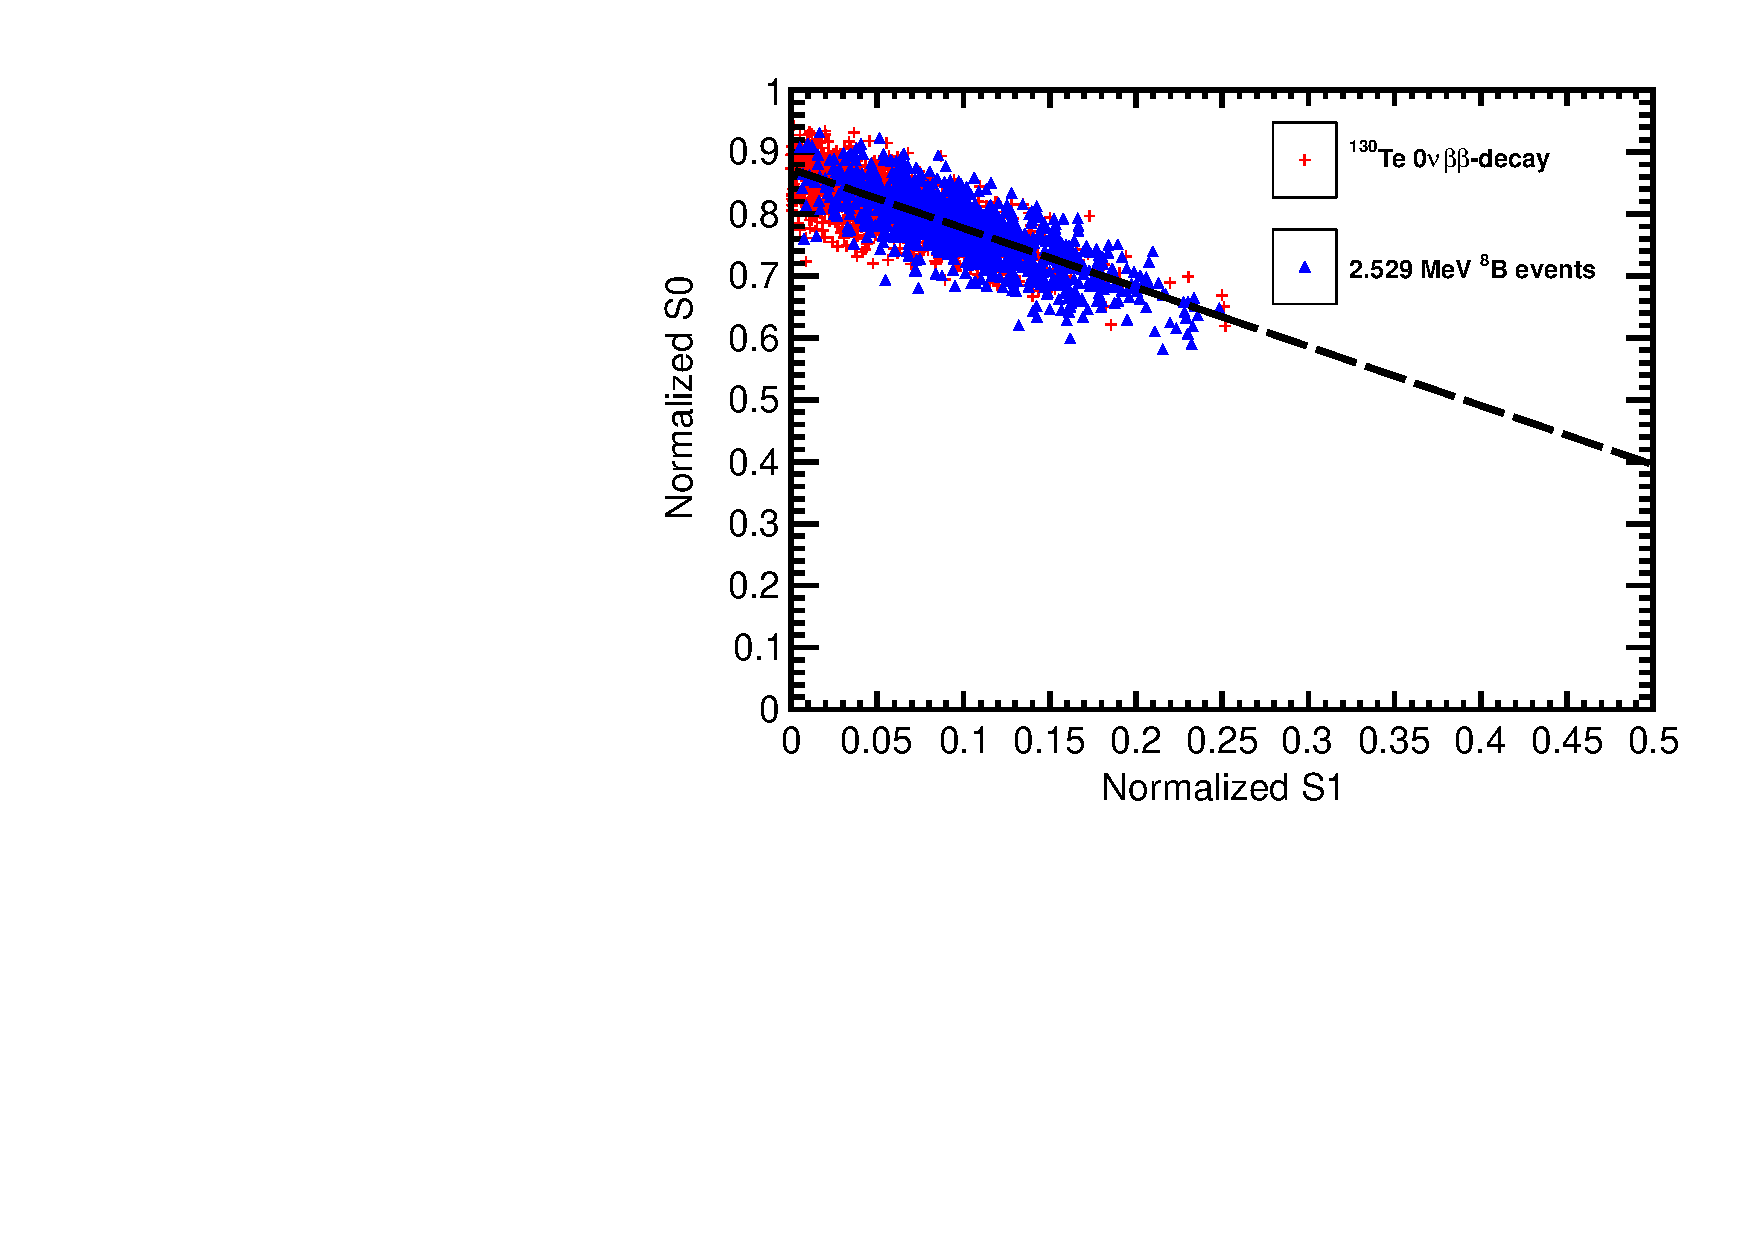
\includegraphics[width=0.49\textwidth]{hS0vsS1_Te130_1el_allLight_VtxSmear0cm_VtxShiftX0cm_momDT1p0ns_rndVtx_3p0mSphere.pdf}
  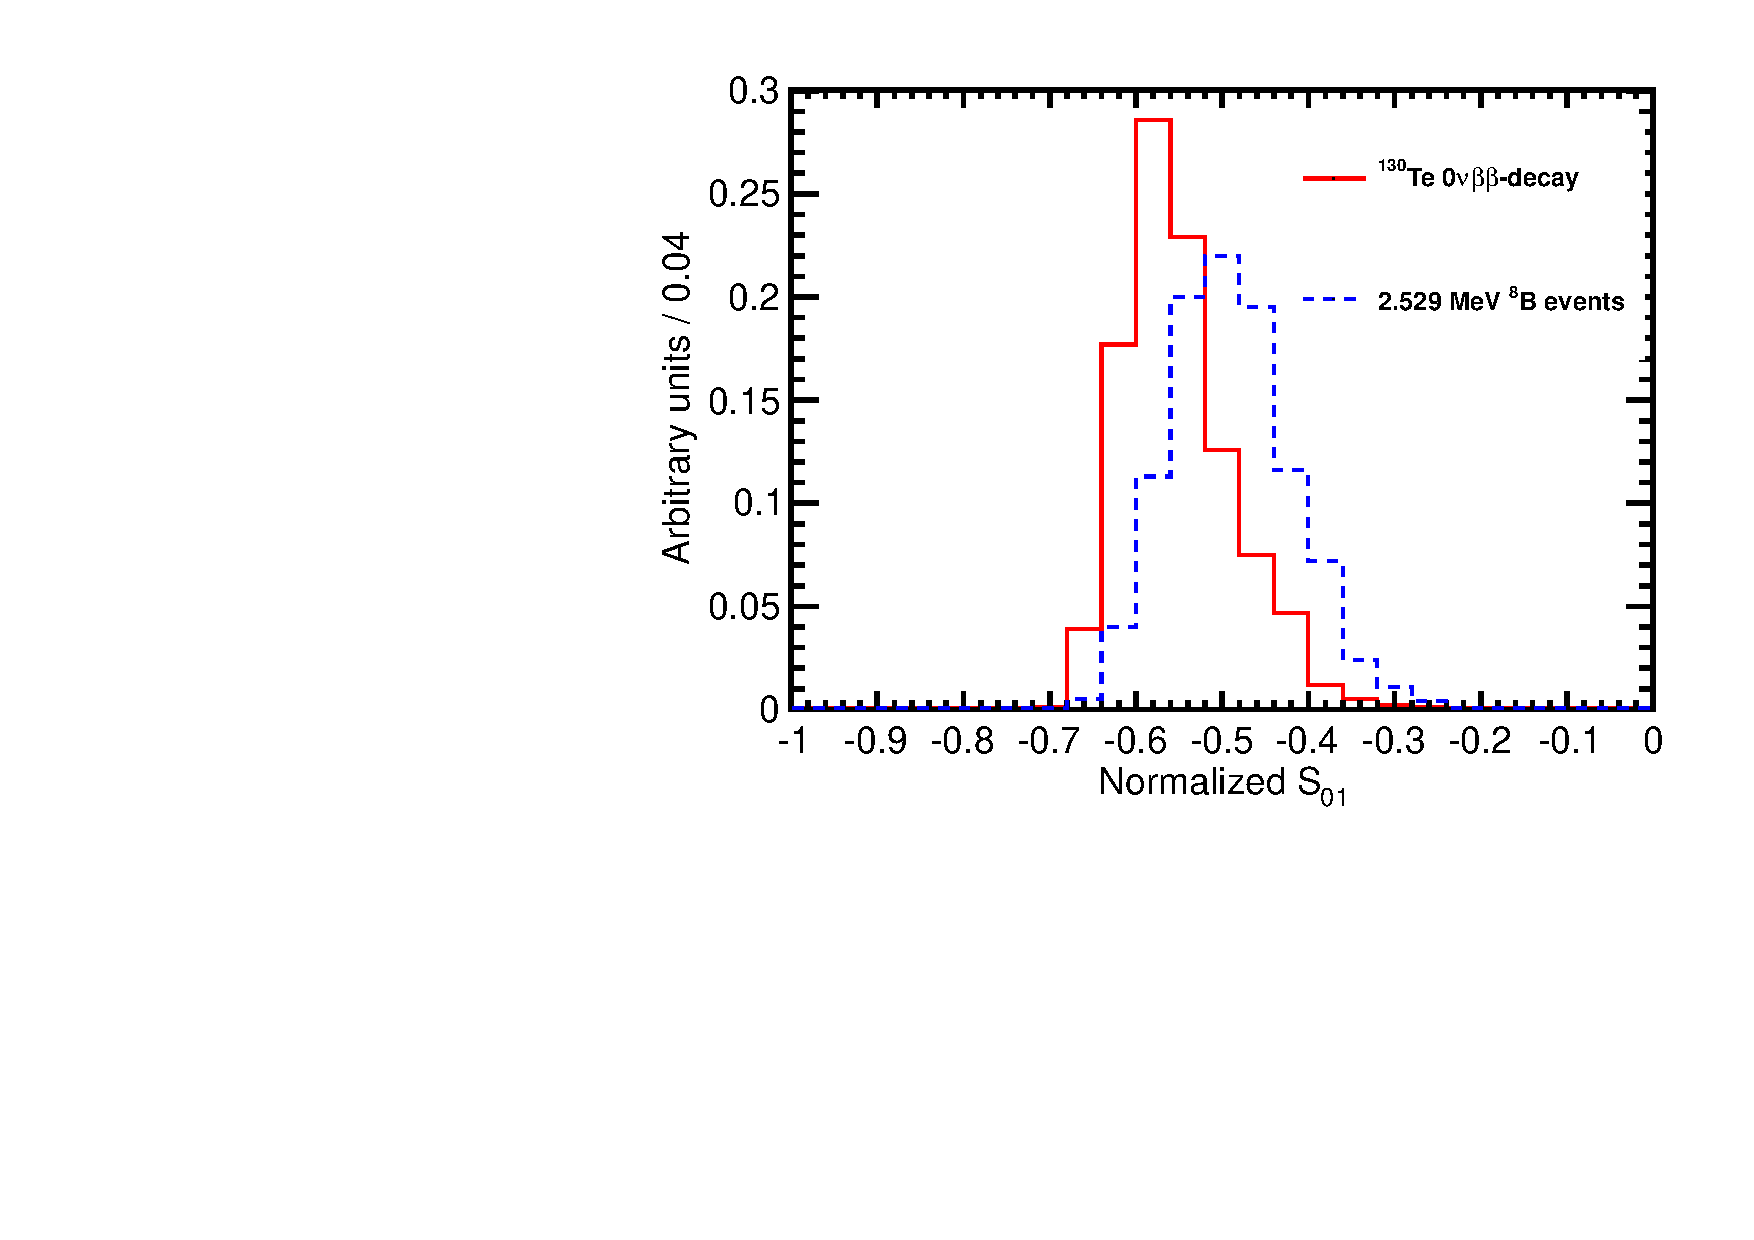
\includegraphics[width=0.49\textwidth]{hS01_allLight_VtxSmear0cm_VtxShiftX0cm_momDT1p0ns_rndVtx_3p0mSphere.pdf}
  \caption{\emph{Left:} Scatter plot of $S_0$ versus $S_1$ for a simulation of 1000 signal (\emph{red crosses}) and background
    (\emph{blue triangles}) events. Event verticies are uniformly distributed within the fiducial volume, $R<3$~m.
    Perfect reconstruction of the vertex position is assumed. Differential cut of 
    $\Delta t=t^{phot}_{measured} - t^{phot}_{predicted}<$1~ns is applied to select early PE sample.
    The default QE and 100\% photo-coverage is used in the simulation.
    Black dashed line corresponds to a linear fit to define 1-D variable $S_{01}$ (see text for details).
    \emph{Right:} Comparison of the $S_{01}$ distribution between signal (\emph{red solid line}) and background (\emph{blue dashed line}).}
  \label{fig:SL_Te_SmearX0cm_momDT1ns_rndVtx_3p0m}
\end{figure*}


\subsubsection{Vertex resolution} 
Imprecise knowledge of the vertex position affects the spherical harmonics analysis in two ways. First, similarly to the effect of chromatic 
dispersion, the vertex uncertainty makes the differential time cut less efficient in separating Cherenkov and scintillation light. 
An uncertainty on the vertex position leads to an uncertainty on the photon predicted travel time, $t^{phot}_{predicted}$, which in turn
increases the probability to mix scintillation and Cherenkov light in the early PE sample.

Second, in the case of single electron event topology, a small error in vertex reconstruction could cause a large effect on the 
normalized power spectrum of spherical harmonics.

Early PE sample of the single electron topology typically has a strong asymmetry due
to preferential directionality of Cherenkov PEs that are selected together with uniformly distributed scintillation PEs. 
Mis-reconstructed vertex introduce asymmetry in the selection of scintillation PE. Vertex shifts parallel to the direction of 
the electron track have the largest effect compared to the shifts in the transverse direction. 

If a vertex is shifted in the direction opposite to the track of the electron, the differential time cut selects more scintillation 
photons that are emitted in the direction of the electron track. Therefore scintillation photons would enhance forward asymmetry of the early PE
sample, which in turn, would move $S_1$ to higher values\footnote{In general, $S_1$ component of the
spherical harmonics power spectrum is higher for asymmetric distributions and lower for symmetric distributions (e.g., compare back-to-back
and single electron topologies in Fig.~\ref{fig:ThreeTopologies_Display_5MeV}). Moreover, $S_1=$~0 for a distribution with perfect symmetry
with respect to the center of the sphere.}.

If a vertex is shifted in the same direction as the direction of the electron, the differential time cut selects more scintillation
photons that are emitted in the direction opposite to the electron track. Therefore, the asymmetry of Cherenkov PEs would be counter
balanced by scintillation PEs, which in turn, would move $S_1$ to lower values.

Figure~\ref{fig:SL_Te_SmearX3cm_momDT1ns_rndVtx_3p0m} shows the performance of the spherical harmonics analysis for events simulated
in the entire fiducial volume with vertex reconstruction resolution of 3~cm. The vertex resolution is implemented
as a substitution of the actual vertex position with a variable that has Gaussian smearing around the actual position along all three
$x-$, $y-$, and $z-$ directions around the actual position. The smearing is done with three independent 
Gaussian distributions that have the same width, $\sigma_x = \sigma_y = \sigma_z =$3~cm.

\begin{figure*}[h]
  \centering
  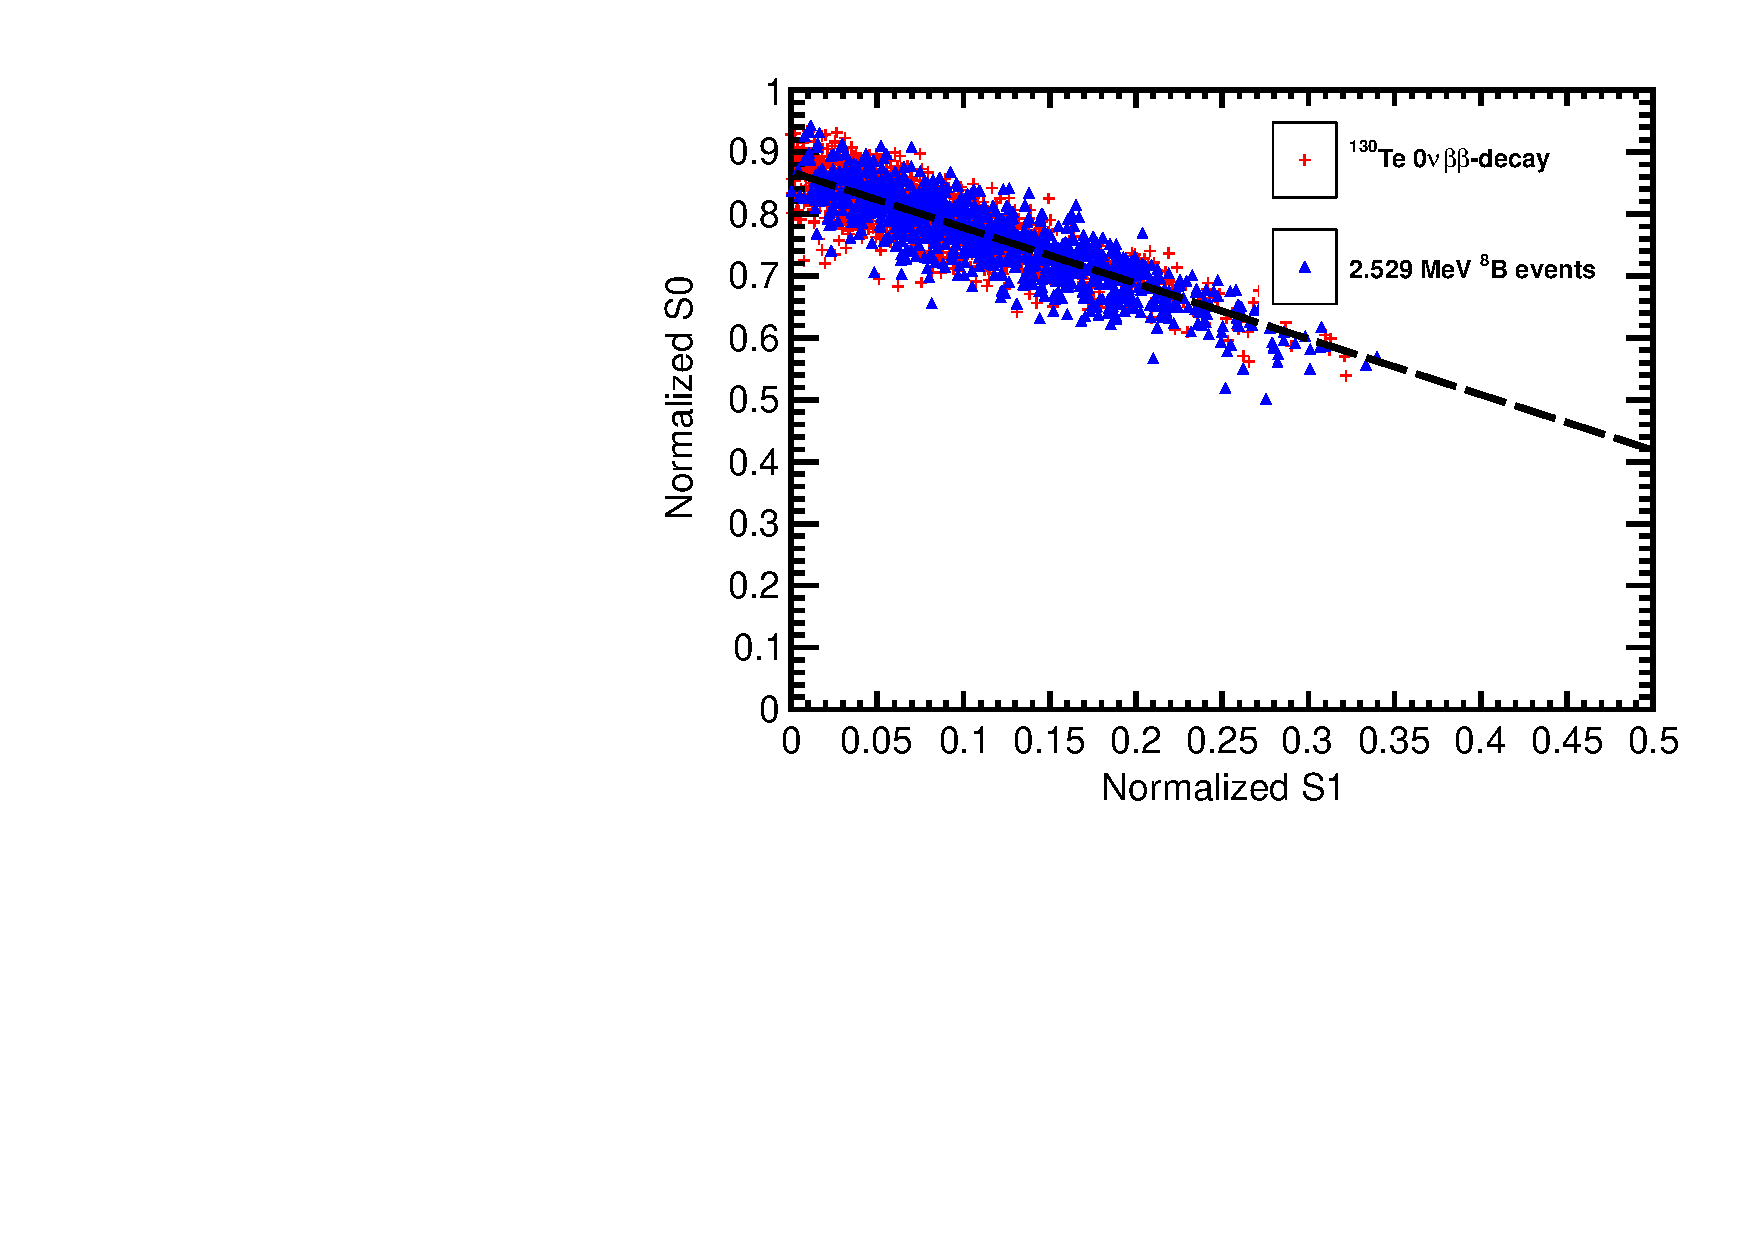
\includegraphics[width=0.49\textwidth]{hS0vsS1_Te130_1el_allLight_VtxSmear3cm_VtxShiftX0cm_momDT1p0ns_rndVtx_3p0mSphere.pdf}
  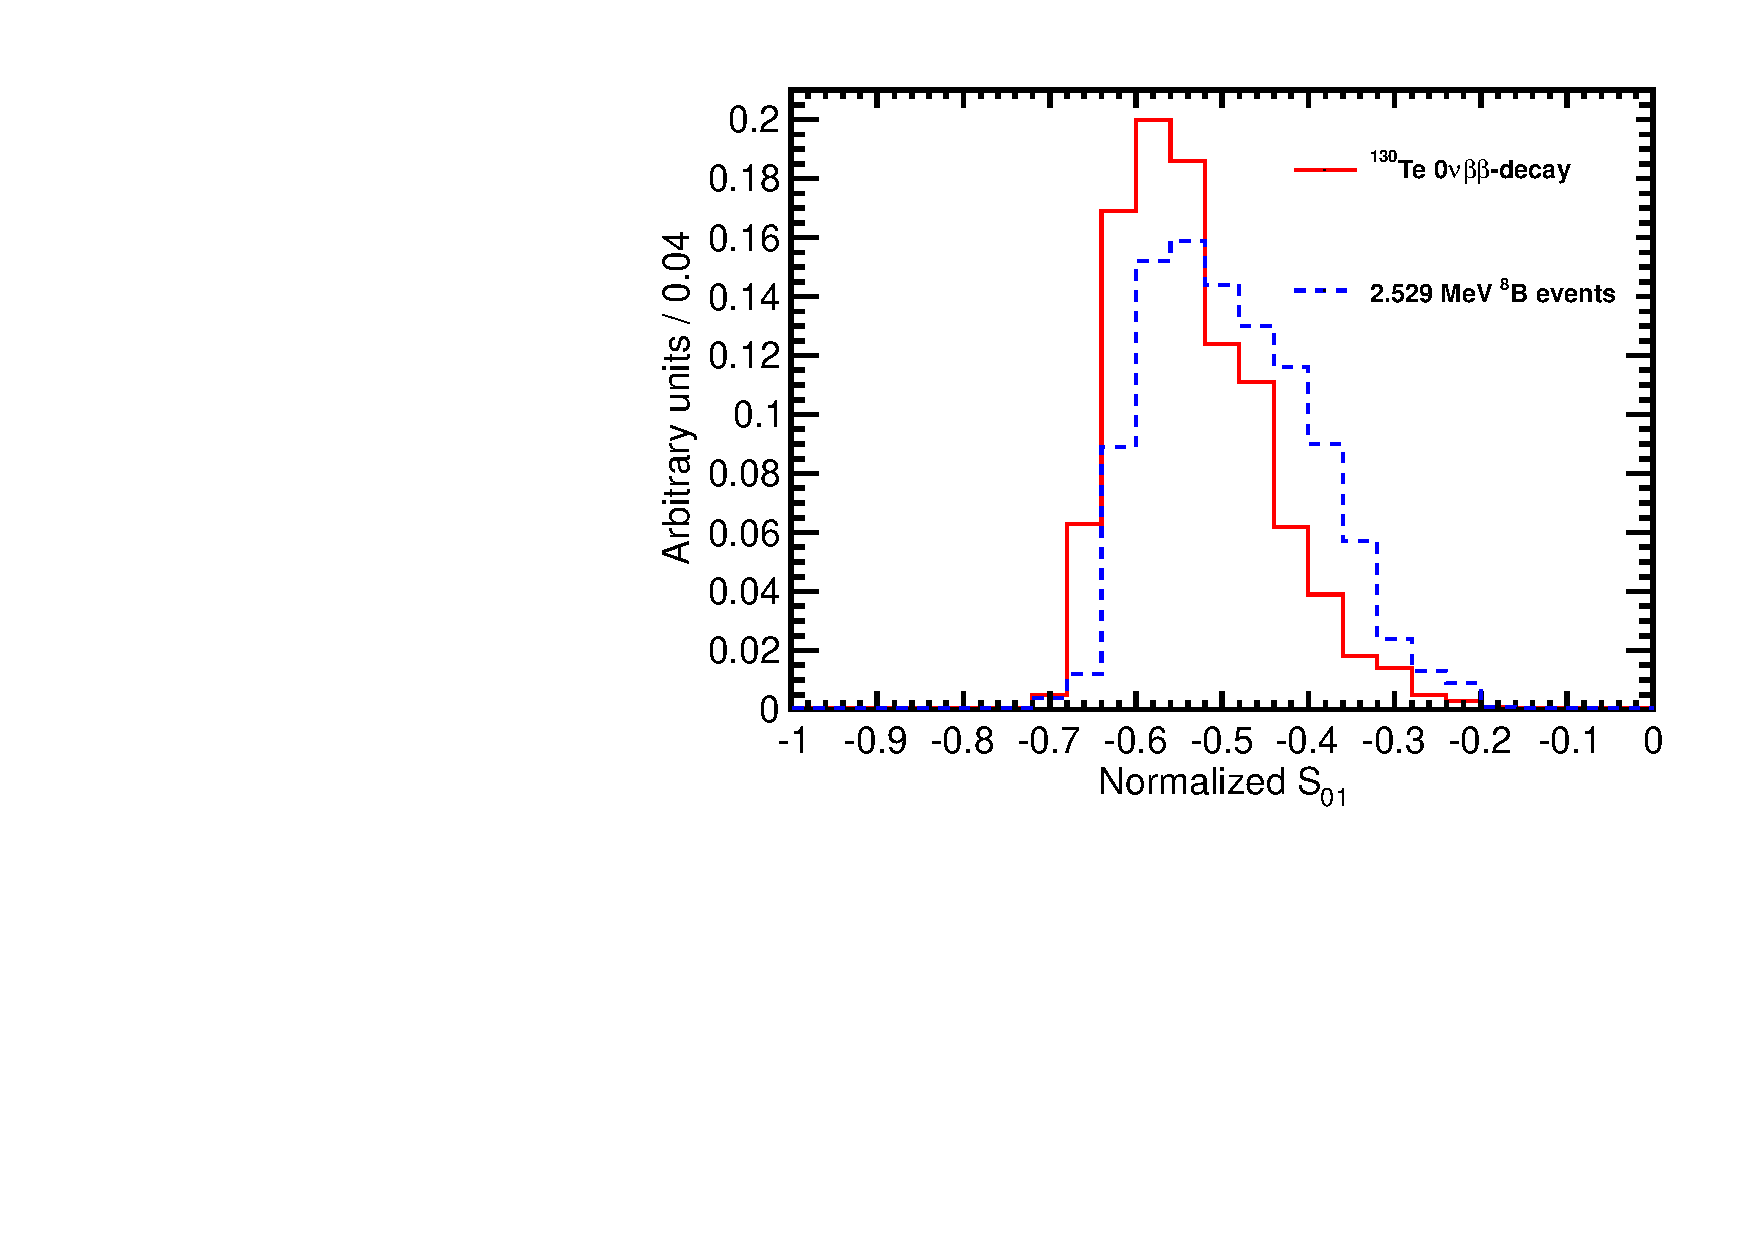
\includegraphics[width=0.49\textwidth]{hS01_allLight_VtxSmear3cm_VtxShiftX0cm_momDT1p0ns_rndVtx_3p0mSphere.pdf}
  \caption{\emph{Left:} Scatter plot of $S_0$ versus $S_1$ for a simulation of 1000 signal (\emph{red crosses}) and background
    (\emph{blue triangles}) events. Event verticies are uniformly distributed within the fiducial volume, $R<3$~m.
    Vertex is smeared with 3~cm resolution. Differential cut of
    $\Delta t=t^{phot}_{measured} - t^{phot}_{predicted}<$1~ns is applied to select early PE sample.
    The default QE and 100\% photo-coverage is used in the simulation.
    Black dashed line corresponds to a linear fit to define 1-D variable $S_{01}$ (see text for details).
    \emph{Right:} Comparison of the $S_{01}$ distribution between signal (\emph{red solid line}) and background (\emph{blue dashed line}).}
\label{fig:SL_Te_SmearX3cm_momDT1ns_rndVtx_3p0m}
\end{figure*}

As can be seen in Fig.~\ref{fig:SL_Te_SmearX3cm_momDT1ns_rndVtx_3p0m}, the vertex resolution effect significantly reduces discrimination power 
of the spherical harmonics analysis in our default detector model.

%{\bf Solution to this problem would be a better selection criteria of
%  early light. It has to preserve high admixture of the Cherenkov
%  photons, but needs to select scintillation photons in a more uniform
%  manner. Working on it, but may not be simple so I don't want to
%  include it in this paper.}


\subsubsection{Requirements for the next generation liquid scintillator detectors}
To take full advantage of topology reconstruction capabilities in the next generation liquid scintillator detectors optical properties of the 
scintillator has to be tuned to allow for better Cherenkov/scintillation light separation.

The effects due to chromatic dispersion can be addressed by using liquid scintillators with a more narrow emission spectrum. For example,
such as described in Ref.~\cite{LS_narrow_emission}.

Strong dependence on the vertex resolution can be addressed by choosing a liquid scintillator mixture with a more delayed emission 
of scintillation light with respect to Cherenkov light. With a larger delay in scintillation light, a high fraction of Cherenkov light 
can be maintained in the early PE sample even if photon track length is mis-reconstructed due to imprecise reconstruction of the vertex 
position. In addition, if the fraction of scintillation light is small compared to Cherenkov light, the distortions in the uniformity of 
the scintillation PE due to shifted reconstructed vertex position would not significantly affect spherical harmonics power spectrum.

While our default detector model assumes scintillation rise time of $\tau_r=$1~ns, scintillation rise time up to $\tau_r=$7~ns can 
be achieved (see Ref.~\ref{Mingfang_slow_rise_time}). As a test we repeated spherical harmonics analysis on 0\nbb-decay and \B~events after
increasing scintillation rise time parameter to $\tau_r=$5~ns in the detector model. All other parameters are kept the same.
Figure ~\ref{fig:SL_Te_SmearX3cm_momDT1ns_rndVtx_3p0m_SciRT5p0ns} shows result of that test. The events are uniformly distributed within 
the fiducial volume and each vertex is smeared with 3~cm resolution. 

We conclude that a rise time of $\tau_r=$5~ns provides sufficient delay between
Cherenkov and scintillation light to make spherical harmonics analysis a potentially useful technique to separate 
0\nbb-decay signal from \B~background.

\begin{figure*}[h]
  \centering
  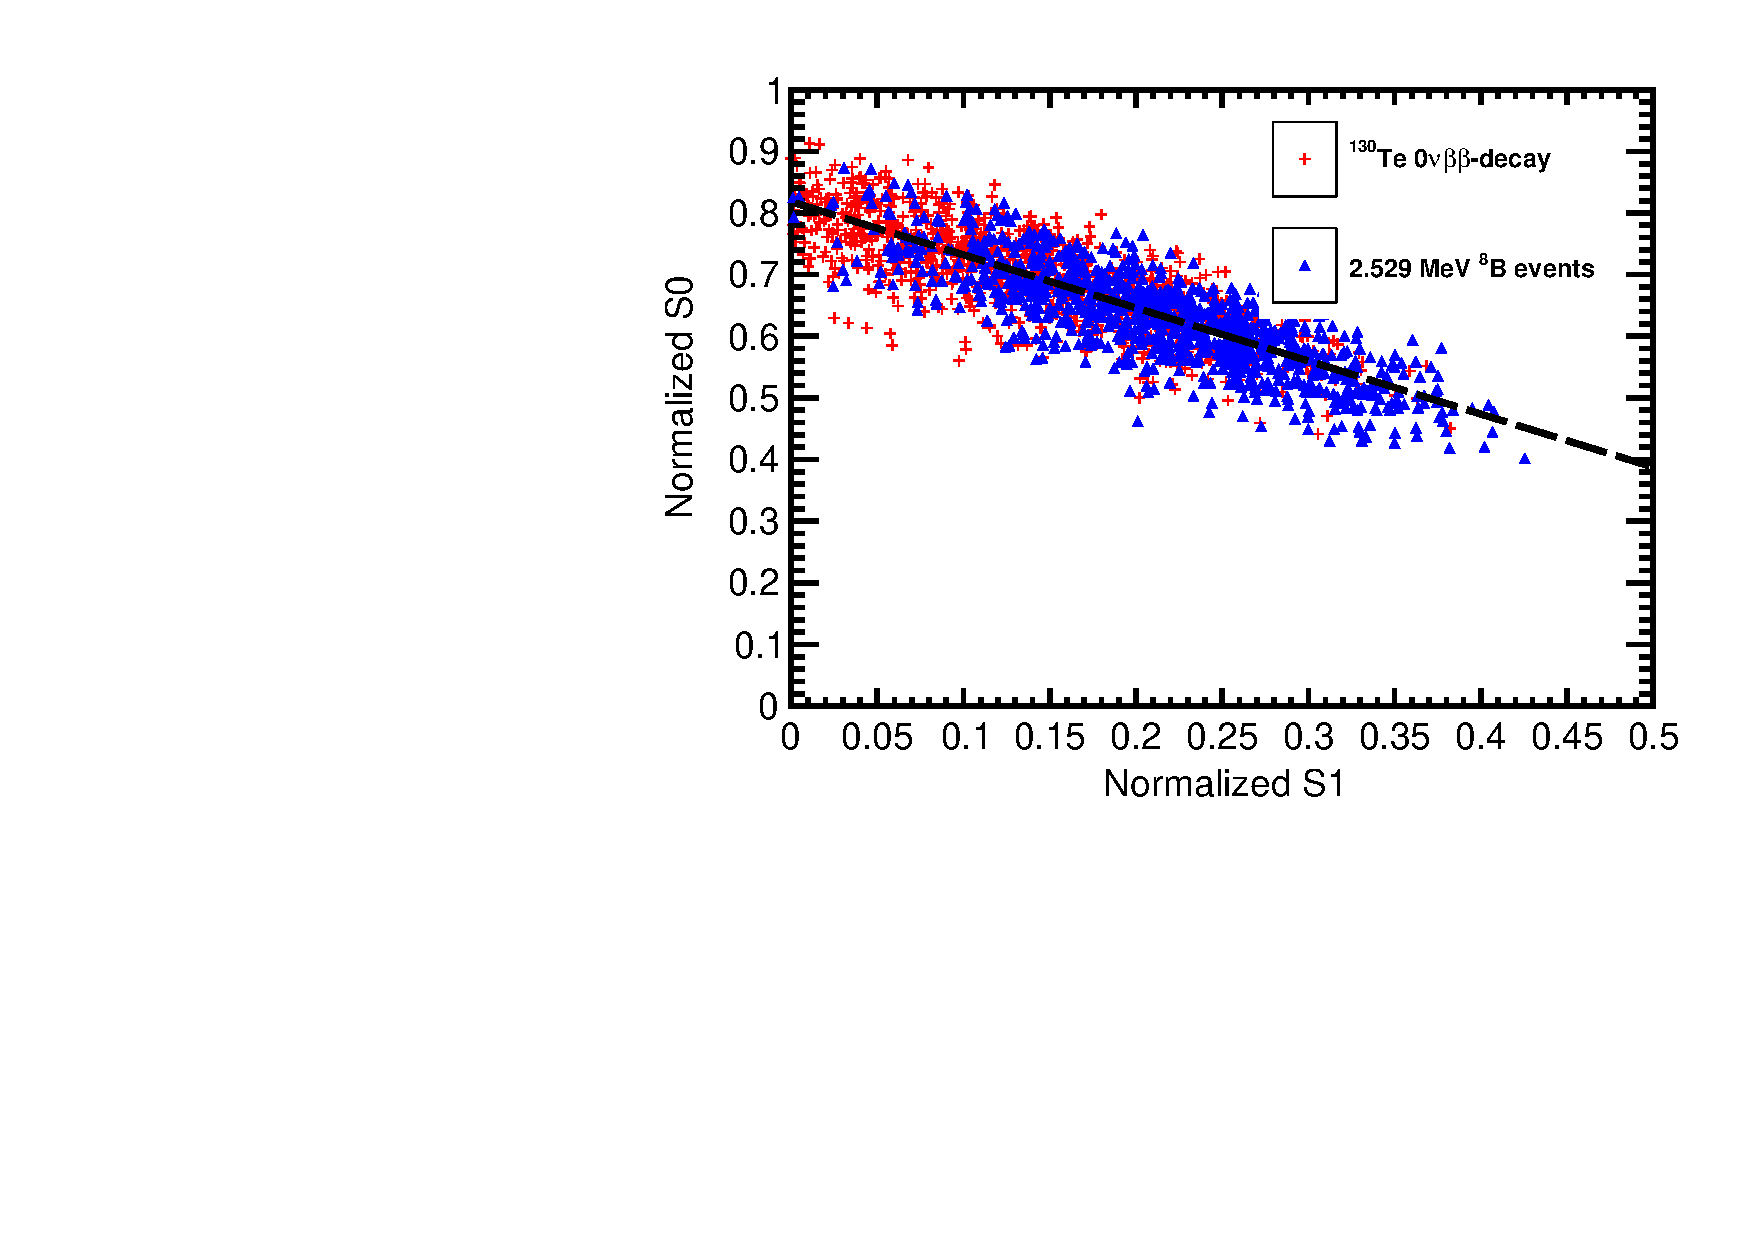
\includegraphics[width=0.49\textwidth]{hS0vsS1_Te130_1el_allLight_VtxSmear3cm_VtxShiftX0cm_momDT1p0ns_rndVtx_3p0mSphere_SciRT5p0ns} 
  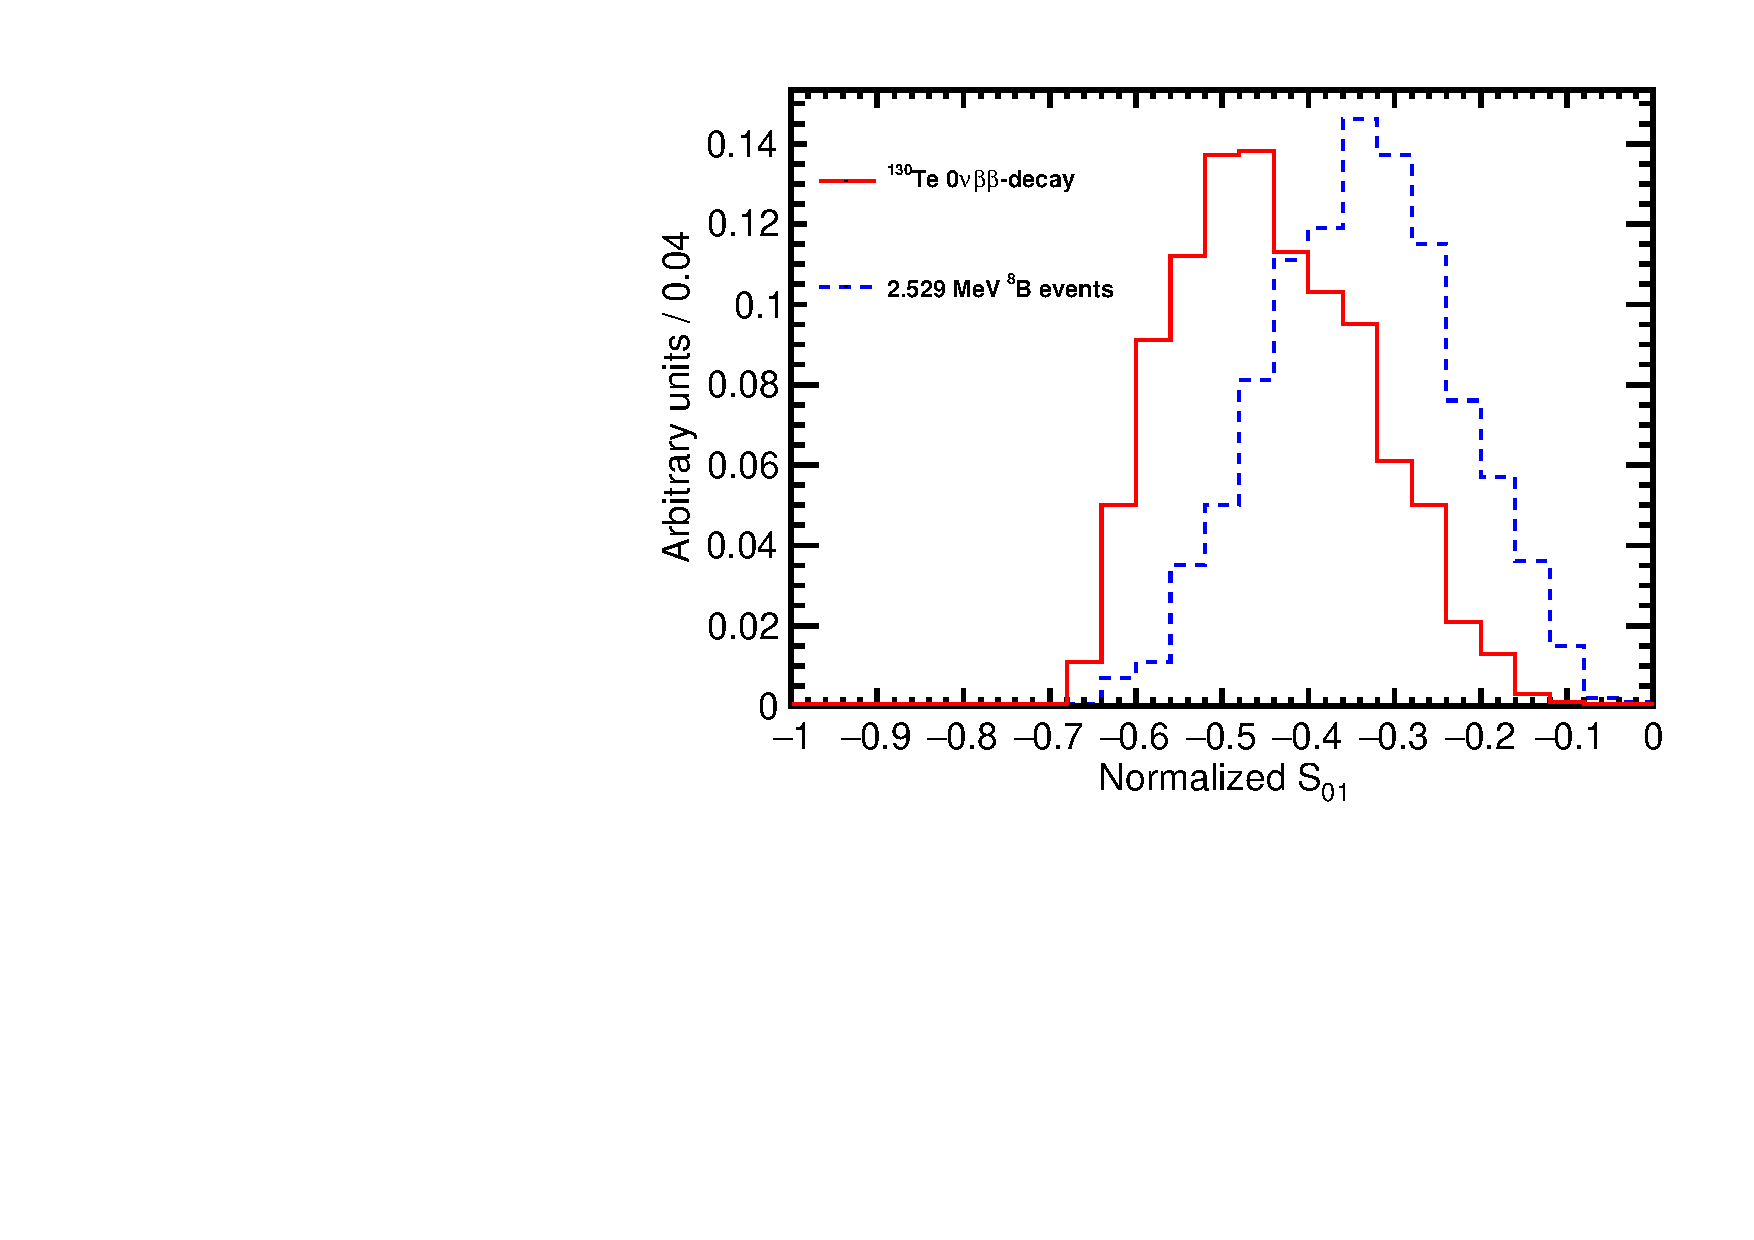
\includegraphics[width=0.49\textwidth]{hS01_allLight_VtxSmear3cm_VtxShiftX0cm_momDT1p0ns_rndVtx_3p0mSphere_SciRT5p0ns}
  \caption{Scintillation rise time constant is increased to $\tau_r=$5~ns compared to $\tau_r=$1~ns in the default detector model.
    \emph{Left:} Scatter plot of $S_0$ versus $S_1$ for a simulation of 1000 signal (\emph{red crosses}) and background
    (\emph{blue triangles}) events. Event verticies are uniformly distributed within the fiducial volume, $R<3$~m.
    Vertex is smeared with 3~cm resolution. Differential cut of
    $\Delta t=t^{phot}_{measured} - t^{phot}_{predicted}<$1~ns is applied to select early PE sample.
    The default QE and 100\% photo-coverage is used in the simulation.
    Black dashed line corresponds to a linear fit to define 1-D variable $S_{01}$ (see text for details).
    \emph{Right:} Comparison of the $S_{01}$ distribution between signal (\emph{red solid line}) and background (\emph{blue dashed line}).}
\label{fig:SL_Te_SmearX3cm_momDT1ns_rndVtx_3p0m_SciRT5p0ns}
\end{figure*}


